The SLAC CRYO \dword{asic} differs from the baseline three-chip design in that it combines the functions of an analog preamplifier, \dword{adc}, and data serialization and transmission for \num{64}~wire channels, into a single chip.
It is based on a design developed for the nEXO experiment\footnote{Enriched Xenon Observatory, \url{https://www-project.slac.stanford.edu/exo/about.html}.} and differs from it only in the design of the preamplifier, which is modified to account for the higher capacitance of the DUNE \dword{spmod} wires compared to the small pads of nEXO.
The \dwords{femb} constructed using this chip would use only two \dwords{asic}, compared to the \num{18} (eight~FE, eight~\dword{adc} and two~COLDATA) needed in the baseline design.
This drastic reduction in part count may significantly improve \dword{femb} reliablity, reduce power, and reduce costs related to production and testing. 

Figure~\ref{fig:cryo-architecture} shows the overall architecture of the CRYO \dword{asic}, which will be implemented in \SI{130}{nm} \dword{cmos}.
It comprises two identical, \num{32}-channel blocks. 
The current signal from each wire is amplified using a preamplifier with pole zero cancellation and an anti-alias fifth-order Bessel filter applied. 
Provisions are also made for injection of test pulses. 
Gain and peaking time are adjustable to values similar to those of the baseline design.

\begin{dunefigure}
[Overall architecture of the CRYO \dword{asic}.]
{fig:cryo-architecture}
{Overall architecture of the CRYO \dword{asic}.}
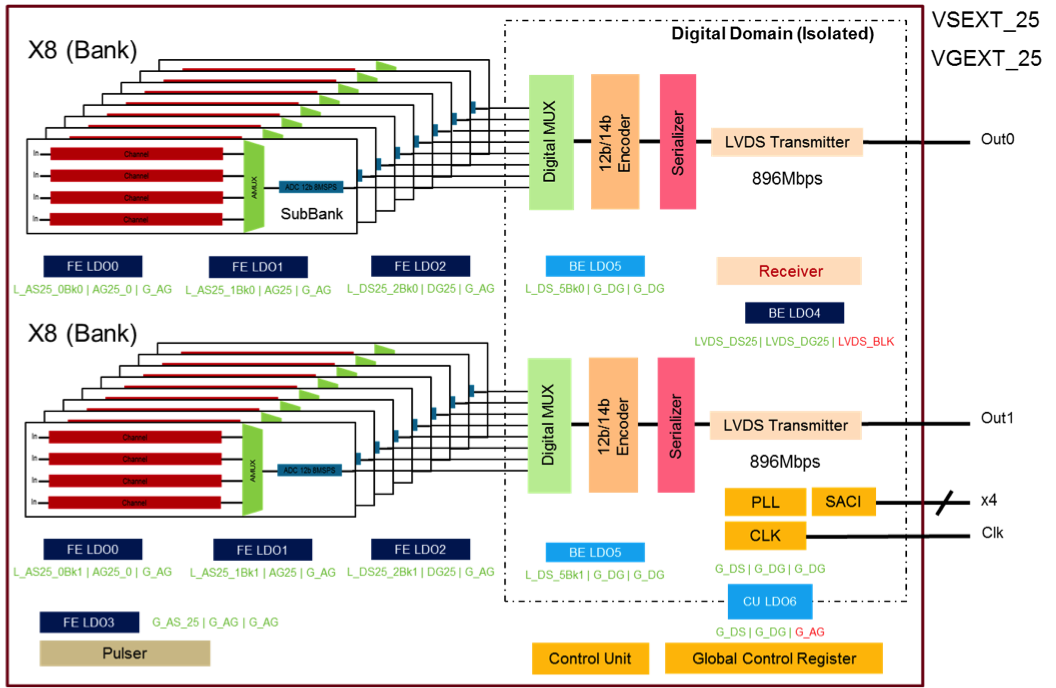
\includegraphics[width=0.8\textwidth]{tpcelec-cryo_schematic.png}
\end{dunefigure}

The \dword{adc} uses \SI{8}{MHz} successive approximation registration (SAR), so that four input channels are multiplexed onto a single \dword{adc}. The data serialization and transmission block employs a custom 12b/14b encoder, so that \num{32} channels of \num{12}-bit, \SI{2}{MHz} data can be transmitted with a digital bandwidth of only \SI{896}{Mbps}, which is significantly less than the required bandwidth of the baseline, which is \SI{1.28}{Gbps}.

One key concern with mixed signal \dwords{asic} is the possibility of interference from the digital side causing noise on the very sensitive preamplifier. 
Fortunately, there are well established techniques for substrate isolation described in the literature~\cite{yeh}, which have been successfully employed in previous \dwords{asic} produced by the SLAC group.% Figure \ref{fig:cryo-substrate} shows how substrate isolation is achieved. 

%\begin{dunefigure}
%[Depiction of the substrate isolation technique that allows combining analog and digital circuitry on the same CRYO \dword{asic}.]
%{fig:cryo-substrate}
%{Depiction of the substrate isolation technique that allows combining analog and digital circuitry on the same CRYO \dword{asic}.}
%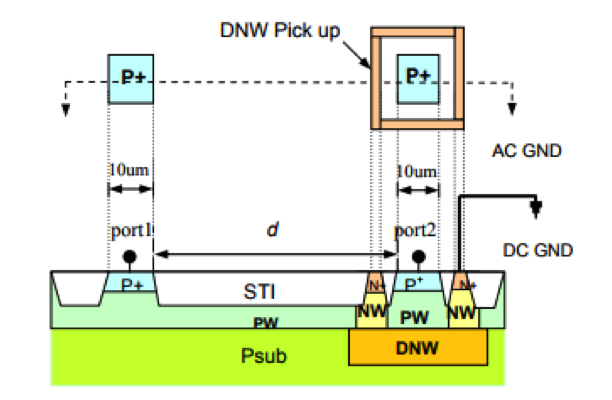
\includegraphics[width=0.6\textwidth]{tpcelec-cryo_substrate.png}
%\end{dunefigure}

The infrastructure requirements for a CYRO \dword{asic}-based system are similar to those of the baseline option. However, in most cases, somewhat fewer resources are needed:
\begin{itemize}
\item{A single voltage is needed for the power supply. This is used to generate two supply voltages using internal voltage regulators.}
\item{The output digital bandwidth on each of the four lines in an \dword{femb} is \SI{896}{Mbps}. This is lower than the baseline option due to the custom 12b/14b encoder of the CRYO chip. }
\item{The warm interface is different. Only a single clock is needed (\SI{56}{MHz}) and the configuration protocol is the SLAC \dword{asic} Control Interface (SACI)~\cite{SACI} rather than I2C.}
\end{itemize}

The first prototype of the CRYO \dword{asic} is in the final design and simulation stages. Simulation-based studies have already been performed; at \SI{0.8}{\micro\second} peaking time and an input capacitance of \SI{200}{pF} (similar to that expected in the DUNE \dword{spmod}), the \dword{enc} is approximately \num{500}\,e$^-$.  This noise level is similar to that expected with the baseline \dword{fe} and \dword{adc} \dword{asic} design in \lar with the same input capacitance.  Submission to the \dword{asic} foundry is imminent and the first prototypes should be received by summer 2018. They will first be tested in an existing test stand at SLAC. Subsequent tests are planned for a small test TPC at \fnal and on an \dword{apa} in the \dword{pdsp} cold box; these test facilities are described in Section~\ref{sec:fdsp-tpc-elec-qa-facilities}.
